\documentclass{extreport}

\usepackage[14pt]{extsizes}
\usepackage[T2A]{fontenc}
\usepackage[utf8]{inputenc}
\usepackage[english,ukrainian]{babel}

\usepackage[a4paper, top=20mm, bottom=20mm, left=30mm, right=20mm]{geometry}
\usepackage{amsmath,amsfonts,amssymb,amsthm,mathtools}
\usepackage{graphicx}
\usepackage{enumitem}
\usepackage{verbatim}
\usepackage{anyfontsize}
\usepackage{indentfirst}
\usepackage{titlesec}

\usepackage{verbatim}
\usepackage{listings}
\usepackage{xcolor}
\definecolor{codegreen}{rgb}{0,0.6,0}
\definecolor{codegray}{rgb}{0.5,0.5,0.5}
\definecolor{codepurple}{rgb}{0.58,0,0.82}
\lstdefinestyle{python_code}{ 
    commentstyle=\color{codegreen},
    keywordstyle=\color{magenta},
    numberstyle=\tiny\color{codegray},
    stringstyle=\color{codepurple},
    basicstyle=\ttfamily\footnotesize,
    breakatwhitespace=false,         
    breaklines=true,                 
    captionpos=b,                    
    keepspaces=true,                            
    numbersep=5pt,                  
    showspaces=false,                
    showstringspaces=false,
    showtabs=false,                  
    tabsize=4
}

\usepackage[psdextra]{hyperref}
\hypersetup{unicode=true}
\hypersetup{
    colorlinks=true,
    linkcolor=blue,
}

\setlist[enumerate]{nosep}
\graphicspath{{pics/}}
\DeclareGraphicsExtensions{.png}

\usepackage{tikz}
\usepackage{pgfplots}
\usepgfplotslibrary{fillbetween}
\pgfplotsset{compat=1.17}

\usetikzlibrary{patterns}
\usetikzlibrary{shapes.geometric}
\usetikzlibrary{arrows.meta}
\usetikzlibrary{shapes.geometric}
\usetikzlibrary{positioning,arrows}
\usetikzlibrary{decorations.markings}
\usetikzlibrary{calc}
\tikzset{
	block/.style={
		draw, 
		rectangle, 
		minimum height=1cm, 
		minimum width=3cm, align=center
	}, 
	line/.style={->,>=stealth'}}
\tikzset{>=latex}

\newcommand\centerarc{} % just for safety
\def\centerarc[#1]#2(#3)#4(#5:#6:#7)% [draw options] (center) (initial angle:final angle:radius)
  {\draw[#1]($(#3)+({#7*cos(#5)},{#7*sin(#5)})$)arc(#5:#6:#7);}

\newcommand{\R}{\mathbb{R}}
\newcommand{\vf}{\varphi}
\renewcommand{\d}[1]{\dot{#1}}
\newcommand{\dd}[1]{\ddot{#1}}
\newcommand{\E}{\mathcal{E}}
\newcommand{\T}{\mathcal{T}}
\newcommand{\bvec}[1]{\boldsymbol{\rm #1}}
\renewcommand{\l}{\left}
\renewcommand{\r}{\right}
\newcommand{\norm}[1]{\left\Vert #1 \right\Vert}
\newcommand{\intl}{\int\limits}
\newcommand{\suml}{\sum\limits}
\newcommand{\dotprod}[2]{\l< #1, #2\r>}
\newcommand{\Lap}[1]{\mathcal{L}\l\{#1\r\}}
\newcommand{\LapInv}[1]{\mathcal{L}^{-1}\l\{#1\r\}}
\def\setdif{\mathbin{\ooalign{\hss\raise1ex\hbox{.}\hss\cr
  \mathsurround=0pt$-$}}}


%\counterwithout{equation}{chapter} 
%\counterwithin*{equation}{section}

\newtheoremstyle{exampstyle}
{3pt} % Space above
{3pt} % Space below
{} % Body font
{} % Indent amount
{\bfseries} % Theorem head font
{.} % Punctuation after theorem head
{.5em} % Space after theorem head
{} % Theorem head spec (can be left empty, meaning `normal')

\theoremstyle{exampstyle}
\newtheorem{definition}{Означення}
\newtheorem*{definition*}{Означення}
\newtheorem{example}{Приклад}[chapter]
\newtheorem*{example*}{Приклад}
\newtheorem{exercise}{Задача}
\newtheorem*{exercise*}{Задача}

\theoremstyle{remark}
\newtheorem*{remark}{Зауваження}

\begin{document}
\begin{titlepage}
    \thispagestyle{empty}
    \begin{center}
        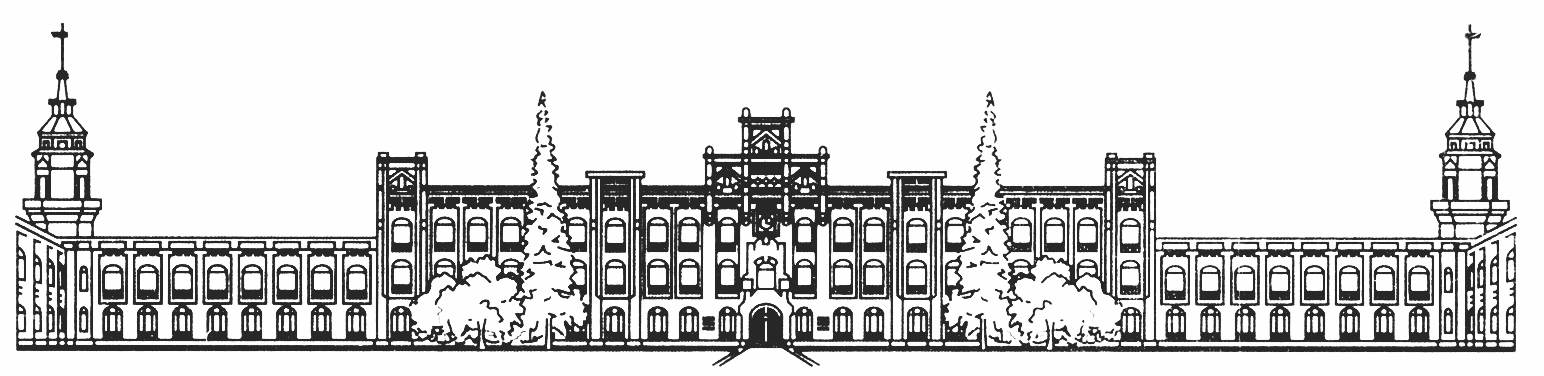
\includegraphics[width = \textwidth]{kpi}
        Міністерство освіти і науки України\\
        Національний технічний університет України\\
        <<Київський політехнічний інститут ім. І. Сікорського>>\\
        Інститут прикладного системного аналізу
    \end{center}
    \vspace{30mm}
    \begin{center}
        \fontsize{22}{26}\selectfont\textbf{Доповідь} \\
        з курсу <<Теорія ігор>> \\
        на тему <<Основи диференціальних ігор. \\ Ігри простого переслідування>>
    \end{center}
    \vspace{30mm}
    \begin{flushleft}
        \textbf{Виконали} \\ 
        студенти 3 курсу групи КА-81 \\
        Галганов Олексій \\
        Фордуй Нікіта
    \end{flushleft}
    \begin{flushright}
        \textbf{Прийняла} \\
        доцент кафедри ММСА \\
        Барановська Леся Валеріївна
    \end{flushright}
    \vspace{30mm}
    \begin{center}
        \textbf{Київ 2021}
    \end{center}
\end{titlepage}
\tableofcontents
    \chapter{Вступ}
        % !TEX root = ../main.tex

\section{Передумови для розгляду диференціальних ігор}
Класична теорія ігор, творцями якої є Джон фон Нейман та Оскар Морґенштерн,
оперує матричними іграми та зв'язаними з ними поняттями. Для них сформульовано та доведено
багато фундаментальних теорем --- наприклад, щодо існування рівноваги Неша. 
Однак, ці результати зовсім не покривають всі можливості формалізувати процеси,
в яких гравці приймають рішення. Наприклад, якщо розглядати задачу про оптимальну траєкторію 
корабля від керованої торпеди, яка його переслідує, то необхідно досліджувати не просто скінченний набір можливих дій
кожного з гравців, а континуум можливих стратегій, кожна з яких відповідає деякій комбінації траєкторій руху корабля та торпеди.

Визначення поняття диференціальної гри буде базуватися на тому, що до їх розв'язання (чи хоча б дослідження)
буде застосовуватися апарат математичного аналізу, як-от теорія диференціальних рівнянь.
Сам термін <<диференціальна гра>> було введено Руфусом Айзексом --- одним з основоположників теорії диференціальних ігор.

Прикладами диференціальних ігор, окрім наведеного вище, є й звичайні спортивні ігри на кшталт футболу,
де, очевидно, недоречно розглядати лише дискретні моменти часу або скінченний набір стратегій,
бо найменше відхилення від таких стратегій (яке, звичайно, може статися через людський фактор),
породжує вже іншу стратегію. Зауважимо, що коли рішення протягом усієї гри приймає лише один гравець,
то така задача фактично стосується \emph{теорії керування} та \emph{варіаційного числення}, тому такі випадки в
теорії ігор не розглядаються. 

\section{Опис ходу гри}
Рішення, що їх приймають гравці, полягають у виборі так званих \emph{керувань}, від яких залежать
\emph{фазові координати}: їх значення у будь-який момент часу повністю визначає хід гри, характеризуючи
положення гравців у деякому просторі --- \emph{фазовому просторі}.
Для визначення результату гри необхідно знати значення фазових координат у початковий момент. Також, в кожен момент часу
гравець має звертати увагу на значення фазових змінних (що, по суті, і означає деяких рух гравців).
В процесі гри фазові координати змінюються. Оскільки розглядається випадок скінченної кількості фазових змінних,
то фазовий простір зручно ототожнювати з координатами точок в $\R^n$ (або в деякій підмножині цього простору).
Поточні значення фазових координат завжди відомі гравцям --- тобто, це ігри з повною інформацією.
Невідомим зазвичай є характер їх зміни: тобто, \emph{керування} фазовими змінними гравцями.
Хід гри характеризується рухом точки у фазовому просторі, причому гра завершується, якщо виконуються деякі умови: наприклад,
потрапляння точки в деяку підмножину простору.

\section{Приклади задання фазових змінних}
Розглянемо приклади задання фазових змінних у випадку керування лише одним об'єктом.
\begin{example}
    Положення матеріальної точки на площині описується двома координатами $x_1$ та $x_2$. 
    Нехай швидкість руху точки є сталою $v$, а гравець обирає напрямок швидкості $\vf$ та може змінювати його у будь-який момент часу --- тобто, $\vf$
    є керуванням. Тоді рух точки описується системою диференціальних рівнянь
    \begin{gather*}
        \begin{cases}
            \d{x_1} = v \cos \vf \\
            \d{x_2} = v \sin \vf
        \end{cases}
    \end{gather*}
    Інший гравець у будь-який момент часу може виміряти значення фазових координат $x_1$ та $x_2$, але закону їх зміни (керування першого гравця) він не знає.
\end{example}
\begin{example}
    Геометричне положення автомобіля на декартовій площині описується трьома фазовими координатами:
    $x_1, x_2$ --- положення деякої точки автомобіля, $x_3$ --- кут, який утворює вісь вздовж автомобіля
    з деяким фіксованим напрямком --- наприклад, $x_1$.
    \begin{center}
        \begin{tikzpicture}
            \draw [->, thick] (-0.5, 0) -- (5, 0);
            \draw [->, thick] (0, -0.5) -- (0, 3);
            \node [below] at (5, 0) {$x_1$};
            \node [left] at (0, 3) {$x_2$};
            \filldraw [fill=lightgray, rounded corners, rotate around={-40:(1,1)}] (1, 1) rectangle (1.7, 2.4);
            \fill [rotate around={-40:(1,1)}] (1.35, 2.4) circle [radius=2pt];
            \draw [->, dashed, rotate around={-40:(1,1)}] (1.35, 0) -- (1.35, 3);
            \draw (0.83, 0) arc (0:44:0.2);
            \draw (0.93, 0) arc (0:45:0.3);
            \node [right] at (0.9, 0.22) {$x_3$};
        \end{tikzpicture}
    \end{center}
    Якщо цей автомобіль є складовою диференціальної гри, то про нього треба знати більше. Нехай гравець керує ним за допомогою педалі акселератора, що
    задає прискорення, та керма, що задає напрямок руху. Нехай $A$ --- максимальне можливе прискорення автомобіля, тоді прискорення може набувати значень
    $A \vf_1$, де $\vf_1 \in [0; 1]$ і знаходиться під контролем гравця-водія. Можна ввести ще одну фазову координату $x_4$ --- швидкість автомобіля.
    Інший гравець у будь-який момент часу знає (чи може виміряти) значення фазових координат, але не значення керування $\vf_1$. Положення керма визначає кривину траєкторії
    руху автомобіля, значення якої, очевидно, є обмеженими. Таким чином, можна ввести кривину як ще одну фазову координату $x_5$
    (фізично --- це кут повороту передніх коліс), керуванням якої є $W \vf_2$, де $\vf_2 \in [-1; 1]$, а $W$ --- максимальна швидкість зміни $x_5$.
    
    Отже, маємо систему, що задає рух автомобіля у деякій диференціальній грі:
    \begin{gather*}
        \begin{cases}
            \d{x_1} = x_4 \cos{x_3} \\
            \d{x_2} = x_4 \sin{x_3} \\
            \d{x_3} = x_4 x_5 \\
            \d{x_4} = A \vf_1, \; \vf_1 \in [0; 1] \\
            \d{x_5} = W \vf_2, \; \vf_2 \in [-1; 1]
        \end{cases}
    \end{gather*}
    Два перших рівняння --- координатний запис швидкості руху автомобіля, третє означає, що швидкість зміни напрямку руху дорівнює добутку швидкості руху на кривину траєкторії,
    а два останні задають керування гравцем швидкості руху та швидкості зміни кривини траєкторії руху. Звісно, вони не є точними з фізичної точки зору (тому що, наприклад, не враховують тертя), але
    є досить простими для аналізу.
\end{example}
    \chapter{Формалізація ігор}
        % !TEX root = ../main.tex

\section{Опис руху}
Вважаємо, що гра відбувається у \emph{фазовому просторі} $\E$ --- деякій області в $\R^n$ та на її межі.
Рух точки $x = \l(x_1, x_2, ..., x_n \r)$ у фазовому просторі описується системою диференціальних рівнянь
\begin{gather}\label{eq_1}
    \begin{cases}
        \d{x_1}(t) = f_1(x_1(t), ..., x_n(t), u_1(x, t), ..., u_P(x, t), v_1(x, t), ..., w_E(x, t)) \\
        \d{x_2}(t) = f_2(x_1(t), ..., x_n(t), u_1(x, t), ..., u_P(x, t), v_1(x, t), ..., w_E(x, t)) \\
        \dots \\
        \d{x_n}(t) = f_n(x_1(t), ..., x_n(t), u_1(x, t), ..., u_P(x, t), v_1(x, t), ..., w_E(x, t)) \\
        x_1(0) = x_1^0, x_2(0) = x_2^0, ..., x_n(0) = x_n^0
    \end{cases}
\end{gather}
або, коротше,
\begin{gather}\label{eq_2}
    \begin{cases}
        \d{x}(t) = {f}(x(t), u(x, t), v(x, t)) \\
        x(0) = x_0
    \end{cases}
\end{gather}
Ці рівняння називаються \emph{рівняннями руху}. Функції $f_j$ є заданими та вважаються достатньо гладкими.
Функції від часу $u$ та $v$ називаються \emph{керуванням} та змінюються, відповідно, першим та другим гравцем, яких
позначатимемо $P$ та $E$. Ці позначення не є випадковими: вони походять від слів pursuer (переслідувач) та evader (утікач), оскільки
саме такі задачі переслідування-втечі дали початок розвитку теорії диференціальних ігор.

Фазові координати $x_1, ..., x_n$ описують стан гри в тому сенсі, що якщо зупинити гру в будь-який момент часу, зафіксувати значення фазових координат
та почати нову гру з цієї зафіксованої точки фазового простору, то її хід буде таким самим, як у початкової гри після моменту зупинки. Зокрема,
значення $x_0$ фазових координат на початку гри, власне, є всім необхідним набором початкових даних, тому, навіть при однакових $f_j$ та керуваннях,
за різних початкових умов отримуватимемо, взагалі кажучи, різні <<партії>> гри.
\begin{example}
    Якщо позначити через $(x_P, y_P)$ координати гравця $P$, через $(x_E, y_E)$ --- гравця $E$, через $w_P$ та $w_E$ їх сталі швидкості руху, 
    а керування напрямком швидкості через $u(t)$ та $v(t)$ відповідно, то отримаємо такі рівняння руху:
    \begin{gather*}
        \begin{cases}
            \d{x_P}(t) = w_P \cos u(t) \\
            \d{y_P}(t) = w_P \sin u(t) \\
            \d{x_E}(t) = w_E \cos v(t) \\
            \d{y_E}(t) = w_E \sin v(t) \\
            (x_P(0), y_P(0)) = (x_P^0, y_P^0) \\
            (x_E(0), y_E(0)) = (x_E^0, y_E^0)
        \end{cases}
    \end{gather*}    
    Такий рух називається <<переслідуванням на площині з простим рухом гравців>>.
\end{example}
\begin{example}[гра <<водій-вбивця>>, \cite{1}]
    В цьому випадку гра також відбувається на площині. Переслідувач $P$ рухається зі сталою швидкістю $w_P$, радіус кривини його траєкторії обмежений
    заданою величиною $R$. Керування $P$ --- це вибір значення кривини в кожний момент часу. Рух утікача $E$ простий: швидкість $w_E$ фіксована,
    керуванням є вибір напрямку швидкості $v(t)$. $E$ в деякому сенсі є більш маневреним, ніж $P$.
    Фазовими координатами в цій грі є пари $x_P, y_P$ і $x_E, y_E$ для опису положення $P$ та $E$ відповідно, та $\theta$ --- напрямок руху $P$.
    \begin{center}
        \begin{tikzpicture}
            \draw [->, thick] (-0.5, 0) -- (7, 0);
            \draw [->, thick] (0, -0.5) -- (0, 5);
            \node [below] at (7, 0) {$x$};
            \node [left] at (0, 5) {$y$};
            % P
            \fill (1.5, 2) circle [radius=2pt];
            \node [below left] at (1.5, 2) {$P$};
            \draw [dashed] (1.5, 2) -- (1.5, 0);
            \draw [dashed] (1.5, 2) -- (0, 2);
            \node [below] at (1.5, 0) {$x_P$};
            \node [left] at (0, 2) {$y_P$};
            \draw (1.5, 2) -- (1.5, 2.7);
            \draw [thick, ->, rotate around={-50:(1.5, 2)}] (1.5, 2) -- (1.5, 3);
            \centerarc[] (1.5, 2) (40:90:0.5);
            \node [above right] at (1.5+0.05, 2+0.35) {$\theta$};
            \draw [thick, rotate around={-50:(1.5, 2)}] (1.5-3, 2) -- (1.5+3.5, 2);
            \fill [rotate around={-50:(1.5, 2)}] (1.5-1.5, 2) circle [radius=2pt];
            \node [below] at (0.4, 3.1) {$C'$};
            \fill [rotate around={-50:(1.5, 2)}] (1.5+1.5, 2) circle [radius=2pt];
            \node [above] at (2.76, 0.71) {$C$};
            \fill [rotate around={-50:(1.5, 2)}] (1.5+2.2, 2) circle [radius=2pt];
            \node [above] at (3.3, 0.1) {$C_1$};
            % E
            \fill (5, 3.5) circle [radius=2pt];
            \node [below left] at (5, 3.5) {$E$};
            \draw [dashed] (5, 3.5) -- (5, 0);
            \draw [dashed] (5, 3.5) -- (0, 3.5);
            \node [below] at (5, 0) {$x_E$};
            \node [left] at (0, 3.5) {$y_E$};
            \draw (5, 3.5) -- (5, 4.2);
            \draw [thick, ->, rotate around={-60:(5, 3.5)}] (5, 3.5) -- (5, 4.5);
            \centerarc[] (5, 3.5) (30:90:0.5);
            \node [above right] at (5+0.05, 3.5+0.35) {$v$};
        \end{tikzpicture}
    \end{center}
    Керування $E$ --- це вибір кута швидкості $v$. Керування $P$ записати дещо складніше. Проведемо через точку $(x_P, y_P)$
    пряму $C' P C$, $|C' P| = |P C| = R$, перпендикулярну до вектору швидкості $P$. $P$ обирає миттєвий центр кривини своєї траєкторії у довільній точці $C_1$ цієї
    прямої, що лежить за межами відрізку $C' C$ (оскільки радіус кривини обмежений). Керування $u(t)$ будемо вважати рівним за модулем
    $R / |P C_1|$, додатним для точок $C_1$, що знаходяться правіше від $P$, та від'ємним для тих, що знаходяться лівіше. Остаточно, маємо такі рівняння руху:
    \begin{gather*}
        \begin{cases}
            \d{x_P}(t) = w_P \sin \theta(t) \\
            \d{y_P}(t) = w_P \cos \theta(t) \\
            \d{x_E}(t) = w_E \sin v(t) \\
            \d{y_E}(t) = w_E \cos v(t) \\
            \d{\theta}(t) = \frac{w_P}{R} u(t), \; u(t) \in [-1; 1]
        \end{cases}
    \end{gather*}
\end{example}

\section{Виграші та стратегії гравців}
Мета диференціальної гри визначається виграшем, який деяким чином
залежить від траєкторій, що пройшли гравці до завершення гри. Позначимо ці траєкторії як функції від часу
як $x(t)$ та $y(t)$. Зауважимо, що диференціальні ігри є \emph{антагоністичними} (або ж, \emph{іграми з нульовою сумою}).

Якщо гра триває деякий заздалегідь визначений час $T$, то виграш гравця $E$ визначається
як $H(x(t), y(T))$, де $H : \R^n \times \R^n \to \R$ --- деяка функція (нагадаємо, що розмірність $\E$ --- $n$). Наприклад, якщо
$$H(x(T), y(T)) = \norm{x(T) - y(T)}$$ то гра описуватиме процес переслідування, в якому
метою гравця $E$ є відхилення від гравця $P$ на момент кінця гри на максимально можливу відстань.
В цьому випадку антагоністичність означає, що метою $P$ є, навпаки, максимальне зближення з $E$ на момент $t=T$. 
Також, можна в якості $H$ використовувати $$H(x(T), y(T)) = \underset{0 \leq t \leq T}{\min} \norm{x(t) - y(t)}$$
Це означатиме, що гравцю $E$ потрібно не просто віддалитися від $P$ в останній момент гри,
а й триматися якнайдалі від $P$ протягом усього часу гри. Це буде так званий \emph{мінімальний виграш}.

Гра також може завершуватися, коли обидва гравці потраплять до деякої підмножини $\T \subset \E$.
Тоді в якості виграшу гравця $E$ можна покласти
$$t_* = \min \l\{ t \geq 0 : (x(t), y(t)) \in \T\r\}$$
$t_*$ --- перший момент потрапляння гравців до $\T$ (або <<захоплення гравцем $P$>>).
Такий виграш називається \emph{термінальним виграшем}. Якщо для всіх $t \geq 0$ вони ніколи не потрапляють до $\T$,
то виграш гравця $E$ дорівнює $+\infty$. Наприклад, якщо в якості $\T$ взяти гіперсферу радіуса $l\geq 0$,
то метою гравця $P$ буде якнайшвидше зближення з $E$ на відстань $l$. Можна також поставити задачу пошуку
таких множин початкових умов, за яких $t_*$ гарантовано буде скінченним або нескінченним. 
В такому випадку можна ввести \emph{якісний виграш}, що набуває значень $\pm 1$ в залежності від того,
чи вдалося $E$ уникнути захоплення гравцем $P$.

\begin{example}(\cite{2})
    Розглянемо переслідування на площині з простим рухом, що описується системою
    \begin{gather*}
        \begin{cases}
            \d{x_1} = u_1, \d{x_2} = u_2, \; u_1^2 + u_2^2 \leq \alpha^2 \\
            \d{y_1} = v_1, \d{y_2} = v_2, \; v_1^2 + v_2^2 \leq \beta^2 \\
            x_1(0) = x_1^0, x_2(0) = x_2^0, y_1(0) = y_1^0, y_2(0) = y_2^0
        \end{cases}
    \end{gather*}
    Тут $P(t) = (x_1, x_2)$ --- координати гравця $P$, $E(t) = (y_1, y_2)$ --- координати гравця $E$.
    $u_1, u_2$ та $v_1, v_2$ --- їх керування відповідно, причому з умови швидкості руху (зміни координат гравців) обмежені
    максимальними значеннями $\alpha$ та $\beta$. Обидва гравці, обираючи керування, змінюють напрямок руху.
    
    Якщо $\alpha > \beta$, то гравець $P$ може гарантувати
    \begin{gather*}
        \forall l \geq 0 : \min \l\{ t \geq 0 : \norm{P(t) - E(t)} \leq l\r\} < +\infty
    \end{gather*}
    тобто, наближення до $E$ на будь-яку відстань за скінченну кількість часу.
    Для цього достатньо рухатися з максимальною швидкістю $\alpha$ в тому ж напрямку, що і $E$.

    Якщо $\alpha \leq \beta$, то в разі $\norm{P(0) - E(0)} > l$ для всіх $l \geq 0$ гравець $E$, рухаючись від $P$ по прямій з максимальною швидкістю,
    зможе уникнути захоплення гравцем $P$.
\end{example}

\begin{definition}
    \emph{Стратегіями} у диференціальній грі є вибір керувань $u$ та $v$ як функцій від часу $t$ та
фазових координат $x$ у системі рівнянь руху (\ref{eq_1}).
\end{definition}
Керування вважаються кусково-гладкими як компроміс між забезпеченням існування розв'язку,
(його може не існувати у класі неперервних функцій) та його єдиності (вона може порушуватися, якщо не вимагати неперервності розв'язку).
Позначатимемо через $\rm P$ та $\rm E$ множини кусково-неперервних стратегій (керувань) гравців $P$ та $E$. 

Надалі для спрощення розглядатимемо не один вектор $x$, а два вектори $x$ та $y$, що відповідатимуть руху кожного з гравців. Тоді
систему (\ref{eq_2}) можна записати як
\begin{gather}\label{eq_3}
    \begin{cases}
        \d{x}(t) = f(x(t), u(x, y, t)) \\
        \d{y}(t) = g(x(t), v(x, y, t)) \\
        x(0) = x_0, y(0) = y_0
    \end{cases}
\end{gather}

\begin{definition}
    Набір $S = \l\{x_0, y_0, u(\cdot), v(\cdot) \r\}$, де $x_0, y_0$ --- початкові умови, а $u \in \rm P$, $v \in \rm E$ --- керування, 
    називається \emph{ситуацією} в диференціальній грі. 
\end{definition}
Якщо розглядати траєкторії, що залежать лише від часу $t$ та накладати на $f$ та $g$ умови
обмеженості та ліпшицевості по $x$ та $y$, тобто
\begin{gather*}
    \norm{f(x_1, u) - f(x_2, u)} \leq \alpha \cdot \norm{x_1 - x_2}, \;
    \norm{g(y_1, v) - g(y_2, v)} \leq \beta \cdot \norm{y_1 - y_2}
\end{gather*}
то за теоремою про існування та єдиність роз'язку задачі Коші, для кожної ситуації $S$ буде існувати єдина пара траєкторій $x(t), y(t)$,
для якої
\begin{gather*}
    \begin{cases}
        \d{x}(t) = f(x(t), u(t)) \\
        \d{y}(t) = g(y(t), v(t)) \\
        x(0) = x_0, y(0) = y_0
    \end{cases}
\end{gather*}

\begin{definition}
    Користуючись означенням ситуації, можна ввести \emph{виграш} в ситуації $S = \l\{x_0, y_0, u(\cdot), v(\cdot) \r\}$
    як функцію $K(x_0, y_0, u(\cdot), v(\cdot))$.
\end{definition}
Приклади виграшів було наведено вище. Траєкторії $x(t)$ та $y(t)$ в них визначаються саме з ситуації $S$. Наведемо строгі означення.
\begin{definition}
        \emph{Термінальний виграш}. Задано деяке число $t>0$ та неперервна по $x$ та $y$ функція $H(x, y)$. Виграш в ситуації $\l\{x_0, y_0, u(\cdot), v(\cdot) \r\}$
        визначається як
        \begin{gather*}
            K(x_0, y_0, u(\cdot), v(\cdot)) = H(x(T), y(T))
        \end{gather*}
        
        \emph{Мінімальний результат}. Задано деяке число $t>0$ та неперервна по $x$ та $y$ функція $H(x, y)$. Виграш в ситуації $\l\{x_0, y_0, u(\cdot), v(\cdot) \r\}$
        визначається як
        \begin{gather*}
            K(x_0, y_0, u(\cdot), v(\cdot)) = \underset{0 \leq t \leq T}{\min} H(x(t), y(t))
        \end{gather*}
        
        \emph{Інтегральний виграш}. Нехай $\T$ --- деяка підмножина $\R^n \times \R^n$, $H(x, y)$ --- неперервна функція. Нехай в ситуації $\l\{x_0, y_0, u(\cdot), v(\cdot) \r\}$
        $t_*$ --- перший момент потрапляння траєкторії $(x(t), y(t))$ на $\T$.
        Тоді
        \begin{gather*}
            K(x_0, y_0, u(\cdot), v(\cdot)) = \intl_0^{t_*} H(x(t), y(t)) dt
        \end{gather*}
        де при $t_* = +\infty$ покладається $K = +\infty$.

        \emph{Якісний виграш}. Нехай $\T$ та $\mathcal{L}$ --- деякі підмножини $\R^n \times \R^n$, а $t_*$ --- перший момент потрапляння траєкторії $(x(t), y(t))$ на $\T$
        в ситуації $\l\{x_0, y_0, u(\cdot), v(\cdot) \r\}$. Тоді
        \begin{gather*}
            K(x_0, y_0, u(\cdot), v(\cdot)) = \begin{cases}
                1, & \text{ якщо } (x(t_*), y(t_*)) \in \mathcal{L} \\
                0, & \text{ якщо } t_* = +\infty \\
                -1, & \text{ якщо } (x(t_*), y(t_*)) \notin \mathcal{L} \\
            \end{cases}
        \end{gather*}
\end{definition}

Нарешті, можна дати означення нормальної форми диференціальної гри.
\begin{definition}
    Нормальною формою диференціальної гри $\Gamma (x_0, y_0)$, заданої на просторі стратегій $\mathrm{P} \times \mathrm{E}$, називається система
    \begin{gather}
        \Gamma (x_0, y_0) = \l<x_0, y_0, \mathrm {P}, \mathrm{E}, K(x_0, y_0, u(\cdot), v(\cdot)) \r>
    \end{gather}
    де $K(x_0, y_0, u(\cdot), v(\cdot))$ --- функція виграшу, визначена будь-який з чотирьох способів вище.
\end{definition}
\begin{remark}
    Кожній парі $(x_0, y_0) \in \R^n \times \R^n$ відповідає своя гра в нормальній формі, тобто, фактично,
    визначається двопараметрична сім'я ігор, що залежать від $(x_0, y_0)$.
\end{remark}
Часто гру називають за функцією виграшу грою з термінальним, інтегральним, якісним виграшем або грою на досягнення мінімального результату.
    \chapter{Ігри з простим рухом}
        % !TEX root = ../main.tex

\section{Простий рух на площині}
Розглянемо найпростіші моделі задач переслідування --- диференціальні ігри на площині з двома учасниками:
переслідувачем $P$ та утікачем $E$, траєкторії яких відповідно позначатимемо $x(t)$ та $y(t)$.
Під \emph{простим рухом} мається на увазі, що закони їх руху описуються системою
\begin{gather}
    \begin{cases}
        \d{x} = u, & \norm{u} \leq \alpha \\
        \d{y} = v, & \norm{v} \leq \beta 
    \end{cases}
\end{gather}
Тут $\norm{z} = \sqrt{z_1^2 + z_2^2}$. Такі закони руху означають, що гравці рухаються з обмеженою швидкістю,
але напрямок руху можуть змінювати довільно. Проінтегрувавши рівняння, можна явно записати траєкторії руху як
\begin{gather*}
    x(t) = x(0) + \intl_0^t u(s) ds, \;
    y(t) = y(0) + \intl_0^t v(s) ds
\end{gather*}
З обмеженості $u$ та $v$ випливає, що 
\begin{gather*}
    \norm{x(t_2) - x(t_1)} \leq \alpha |t_2 - t_1|, \;
    \norm{y(t_2) - y(t_1)} \leq \beta |t_2 - t_1|
\end{gather*}

\begin{example}
    Нехай $u(t) = \begin{pmatrix} -\sin t \\ 2 \cos {2t}\end{pmatrix}$, 
    $v(t) = \begin{pmatrix} -\sqrt{2}\sin t \\ \sqrt{2}\cos t \end{pmatrix}$,
    $x(0) = \begin{pmatrix} 1 \\ 0 \end{pmatrix}$, 
    $y(0) = \begin{pmatrix} \sqrt{2} \\ 0 \end{pmatrix}$, 
    а гра триває до моменту $T = 2\pi$.
    Знайти значення функції виграшу мінімального результату з $H(x, y) = \norm{x - y}$.

    Знайдемо рівняння траєкторій:
    \begin{gather*}
        x(t) = \begin{pmatrix} 1 \\ 0 \end{pmatrix} +
        \intl_0^t \begin{pmatrix} -\sin s \\ 2 \cos {2s} \end{pmatrix} ds = 
        \begin{pmatrix} 1 \\ 0 \end{pmatrix} +
        \l.\begin{pmatrix} \cos s \\ \sin{2s} \end{pmatrix}\r|_0^t = 
        \begin{pmatrix} \cos t \\ \sin{2t} \end{pmatrix}
    \end{gather*}
    \begin{gather*}
        y(t) = \begin{pmatrix} \sqrt{2} \\ 0 \end{pmatrix} +
        \intl_0^t \begin{pmatrix} -\sqrt{2}\sin s \\ \sqrt{2}\cos s  \end{pmatrix} ds = 
        \begin{pmatrix} \sqrt{2}\cos t \\ \sqrt{2}\sin t \end{pmatrix}
    \end{gather*}
    \begin{center}
        \begin{tikzpicture}
        \begin{axis}
            [axis lines = center,
            axis equal,
            trig format plots=rad,
            xmin=-1.5, xmax=1.5, ymin=-1.5, ymax=1.5,
            legend pos = outer north east]
            \addplot [
                domain=0:2*pi,
                samples=100,
                color=red,
                decoration={markings, mark=between positions 0.05 and 0.1 step 2em with {\arrow [scale=1.5]{stealth}}
                }, postaction=decorate, forget plot
            ] ({cos(x)}, {sin(2*x)});
            \addlegendimage{red}
            \addlegendentry{$x(t)$}
            \addplot [
                domain=0:2*pi,
                samples=100,
                color=green,
                decoration={markings, mark=between positions 0.05 and 0.1 step 2em with {\arrow [scale=1.5]{stealth}}
                }, postaction=decorate, forget plot
            ] ({sqrt(2)*cos(x)}, {sqrt(2)*sin(x)});
            \addlegendimage{green}
            \addlegendentry{$y(t)$}
        \end{axis}
    \end{tikzpicture}
    \end{center}
    Значення $K = \underset{0 \leq t \leq 2\pi}{\min} \norm{x(t) - y(t)}$ можна знайти чисельно:
    $K \approx 0.282394$ при $t \approx 0.850448$.
\end{example}

\section{Простий рух в \texorpdfstring{$\R^n$}{Rn}}\label{sec_3_2}
Тепер розглянемо гру переслідування вже не на площині $\R^2$, а в $\R^n$:
\begin{gather}
    \begin{cases}
        \d{x} = u, & \norm{u} \leq \alpha \\
        \d{y} = v, & \norm{v} \leq \beta \\
        x(0) = x_0, \; y(0) = y_0
    \end{cases}
\end{gather}
Тут усі величини є $n$-вимірними векторами, і, як раніше, $x(t)$ --- траєкторія
руху переслідувача $P$, $y(t)$ --- утікача $E$.

Нехай $\alpha > \beta$, тобто, переслідувач може рухатися швидше за утікача. Дослідимо,
чи зможе $P$ наздогнати $E$ та, якщо зможе, як йому потрібно рухатися (за матеріалом в \cite{3}).
Нехай $z = x - y$, тоді маємо систему
\begin{gather*}
    \d{z} = u - v \\
    z(0) = z_0 = x_0 - y_0
\end{gather*}
$P$ може наздогнати $E$, якщо $\exists T < +\infty : z(T) = 0 \Leftrightarrow \norm{z(T)} = 0$.
Введемо функцію $f(t) = \norm{z(t)}^2 = z_1^2(t) + ... + z_n^2(t)$ та дослідимо її похідну.
\begin{gather*}
    \d{f}(t) = 2 z_1(t) \d{z_1}(t) +  ... + 2 z_n(t) \d{z_n}(t) =
    2 \dotprod{z(t)}{\d{z}(t)} = \\ = 2 \l(\dotprod{z(t)}{u(t)} - \dotprod{z(t)}{v(t)} \r)
\end{gather*}
Якщо $u(t) = - \frac{\alpha}{\norm{z(t)}} z(t)$, то 
\begin{gather*}
    \d{f}(t) = 2 \l( -\alpha \norm{z(t)} - \dotprod{z(t)}{v(t)}\r) \leq
    2 \l( -\alpha \norm{z(t)} + \norm{z(t)}\cdot \norm{v(t)}\r) \leq \\
    \leq 2 \l( -\alpha \norm{z(t)} + \beta \norm{z(t)}\r) = 2(\beta - \alpha) \norm{z(t)} = 
    2 (\beta - \alpha) \sqrt{f(t)}
\end{gather*}
Проінтегрувавши від $0$ до $t$ нерівність $\frac{\d{f}(t)}{2\sqrt{f(t)}} \leq \beta - \alpha$,
отримаємо
\begin{gather*}
    \sqrt{f(t)} - \sqrt{f(0)} \leq (\beta - \alpha) t \Leftrightarrow
    \norm{z(t)} - \norm{z(0)} \leq (\beta - \alpha) t \Leftrightarrow \\ \Leftrightarrow
    \norm{z(t)} \leq \norm{z(0)} + (\beta - \alpha) t
\end{gather*}
Оскільки при $t = \frac{\norm{z(0)}}{\alpha - \beta}$ права частина отриманої нерівності дорівнює 0.
Тому, як би не рухався $E$, момент, коли $P$ його наздожене, наступить не пізніше $T(z_0) = \frac{\norm{z_0}}{\alpha - \beta}$.
З іншого боку, якщо $E$ обиратиме $v(t) = -\frac{\beta}{\norm{z(t)}} z(t)$, то
\begin{gather*}
    \d{f}(t) = 2 \l(-\alpha \norm{z(t)} + \beta \norm{z(t)}\r) = 2(\beta - \alpha) \sqrt{f(t)}
\end{gather*}
Інтегруванням отримаємо
\begin{gather*}
    \norm{z(t)} = \norm{z(0)} - (\alpha - \beta) t
\end{gather*}
і тому момент, коли $P$ наздожене $E$, наступить не раніше $T(z_0)$.

Таким чином, яку б стратегію $v(t)$ не обрав утікач $E$, переслідувач $P$ наздожене його не пізніше,
ніж за $\frac{\norm{x_0 - y_0}}{\alpha - \beta}$, використовуючи стратегію $u(t) = - \frac{\alpha}{\norm{x(t) - y(t)}} (x(t) - y(t))$,
причому переслідування буде найдовшим, якщо $E$ обере <<раціональну>> стратегію $v(t) = - \frac{\beta}{\norm{x(t) - y(t)}} (x(t) - y(t))$.

\begin{example}\label{ex_3_2}
    Перевіримо отримані твердження на прикладах. Нехай $n=1$ (переслідування на прямій), $\alpha = 3, \beta = 1$, гра починається з $x_0 = 0$ та $y_0 = 1$ і обидва гравці обирають стратегії, вказані вище.
    Розв'яжемо чисельно (методом Рунге-Кутта) відповідну систему диференціальних рівнянь і подивимося на графіки $x(t)$ та $y(t)$ в залежності від часу.
    Видно, що $P$ дійсно наздогнав $E$ у момент $T = \frac{|0 - 1|}{3 - 1} = 0.5$.
    \begin{center}
        % This file was created by tikzplotlib v0.9.8.
\begin{tikzpicture}

\begin{axis}[
legend cell align={left},
legend style={
  fill opacity=0.8,
  draw opacity=1,
  text opacity=1,
  at={(0.03,0.97)},
  anchor=north west,
  draw=white!80!black
},
tick align=outside,
tick pos=left,
x grid style={white!69.0196078431373!black},
xlabel={\(\displaystyle t\)},
xmin=-0.0275, xmax=0.5775,
xtick style={color=black},
y grid style={white!69.0196078431373!black},
ymin=-0.0748333333333333, ymax=1.5715,
ytick style={color=black}
]
\addplot [semithick, red]
table {%
0 0
0.01 0.03
0.02 0.06
0.03 0.09
0.04 0.12
0.05 0.15
0.06 0.18
0.07 0.21
0.08 0.24
0.09 0.27
0.1 0.3
0.11 0.33
0.12 0.36
0.13 0.39
0.14 0.42
0.15 0.45
0.16 0.48
0.17 0.51
0.18 0.54
0.19 0.57
0.2 0.6
0.21 0.63
0.22 0.66
0.23 0.69
0.24 0.72
0.25 0.75
0.26 0.78
0.27 0.81
0.28 0.840000000000001
0.29 0.870000000000001
0.3 0.900000000000001
0.31 0.930000000000001
0.32 0.960000000000001
0.33 0.990000000000001
0.34 1.02
0.35 1.05
0.36 1.08
0.37 1.11
0.38 1.14
0.39 1.17
0.4 1.2
0.41 1.23
0.42 1.26
0.43 1.29
0.44 1.32
0.45 1.35
0.46 1.38
0.47 1.41
0.48 1.44
0.49 1.47
0.5 1.49
0.51 1.49
0.52 1.49
0.53 1.49
0.54 1.49
0.55 1.49
};
\addlegendentry{$x(t)$}
\addplot [semithick, green]
table {%
0 1
0.01 1.01
0.02 1.02
0.03 1.03
0.04 1.04
0.05 1.05
0.06 1.06
0.07 1.07
0.08 1.08
0.09 1.09
0.1 1.1
0.11 1.11
0.12 1.12
0.13 1.13
0.14 1.14
0.15 1.15
0.16 1.16
0.17 1.17
0.18 1.18
0.19 1.19
0.2 1.2
0.21 1.21
0.22 1.22
0.23 1.23
0.24 1.24
0.25 1.25
0.26 1.26
0.27 1.27
0.28 1.28
0.29 1.29
0.3 1.3
0.31 1.31
0.32 1.32
0.33 1.33
0.34 1.34
0.35 1.35
0.36 1.36
0.37 1.37
0.38 1.38
0.39 1.39
0.4 1.4
0.41 1.41
0.42 1.42
0.43 1.43
0.44 1.44
0.45 1.45
0.46 1.46
0.47 1.47
0.48 1.48
0.49 1.49
0.5 1.49666666666667
0.51 1.49666666666667
0.52 1.49666666666667
0.53 1.49666666666667
0.54 1.49666666666667
0.55 1.49666666666667
};
\addlegendentry{$y(t)$}
\addplot [semithick, black, dashed, forget plot]
table {%
0.5 -0.0748333333333334
0.5 1.5715
};
\end{axis}

\end{tikzpicture}

    \end{center}

    Нехай тепер переслідування відбувається на площині ($n=2$), обмеження швидкостей ті ж самі, гра починається з $x_0 = \begin{pmatrix}
        0 \\ 0
    \end{pmatrix}$ та $y_0 = \begin{pmatrix}
        1 \\ 1
    \end{pmatrix}$.
    \begin{center}
        % This file was created by tikzplotlib v0.9.8.
\begin{tikzpicture}

\begin{axis}[
legend cell align={left},
legend style={
  fill opacity=0.8,
  draw opacity=1,
  text opacity=1,
  at={(0.03,0.97)},
  anchor=north west,
  draw=white!80!black
},
tick align=outside,
tick pos=left,
x grid style={white!69.0196078431373!black},
xmin=-0.0749844396019248, xmax=1.57467323164042,
xtick style={color=black},
y grid style={white!69.0196078431373!black},
ymin=-0.0749844396019248, ymax=1.57467323164042,
ytick style={color=black}
]
\addplot [semithick, red, opacity=0.5]
table {%
0 0
0.0212132034355964 0.0212132034355964
0.0424264068711929 0.0424264068711929
0.0636396103067893 0.0636396103067893
0.0848528137423857 0.0848528137423857
0.106066017177982 0.106066017177982
0.127279220613579 0.127279220613579
0.148492424049175 0.148492424049175
0.169705627484771 0.169705627484771
0.190918830920368 0.190918830920368
0.212132034355964 0.212132034355964
0.233345237791561 0.233345237791561
0.254558441227157 0.254558441227157
0.275771644662754 0.275771644662754
0.29698484809835 0.29698484809835
0.318198051533946 0.318198051533946
0.339411254969543 0.339411254969543
0.360624458405139 0.360624458405139
0.381837661840736 0.381837661840736
0.403050865276332 0.403050865276332
0.424264068711928 0.424264068711928
0.445477272147525 0.445477272147525
0.466690475583121 0.466690475583121
0.487903679018718 0.487903679018718
0.509116882454314 0.509116882454314
0.53033008588991 0.53033008588991
0.551543289325507 0.551543289325507
0.572756492761103 0.572756492761103
0.5939696961967 0.5939696961967
0.615182899632296 0.615182899632296
0.636396103067893 0.636396103067893
0.657609306503489 0.657609306503489
0.678822509939085 0.678822509939085
0.700035713374682 0.700035713374682
0.721248916810278 0.721248916810278
0.742462120245875 0.742462120245875
0.763675323681471 0.763675323681471
0.784888527117067 0.784888527117067
0.806101730552664 0.806101730552664
0.82731493398826 0.82731493398826
0.848528137423857 0.848528137423857
0.869741340859453 0.869741340859453
0.890954544295049 0.890954544295049
0.912167747730646 0.912167747730646
0.933380951166242 0.933380951166242
0.954594154601839 0.954594154601839
0.975807358037435 0.975807358037435
0.997020561473031 0.997020561473031
1.01823376490863 1.01823376490863
1.03944696834422 1.03944696834422
1.06066017177982 1.06066017177982
1.08187337521542 1.08187337521542
1.10308657865101 1.10308657865101
1.12429978208661 1.12429978208661
1.14551298552221 1.14551298552221
1.1667261889578 1.1667261889578
1.1879393923934 1.1879393923934
1.209152595829 1.209152595829
1.23036579926459 1.23036579926459
1.25157900270019 1.25157900270019
1.27279220613579 1.27279220613579
1.29400540957138 1.29400540957138
1.31521861300698 1.31521861300698
1.33643181644258 1.33643181644258
1.35764501987817 1.35764501987817
1.37885822331377 1.37885822331377
1.40007142674937 1.40007142674937
1.42128463018496 1.42128463018496
1.44249783362056 1.44249783362056
1.46371103705615 1.46371103705615
1.48492424049175 1.48492424049175
1.49906637611548 1.49906637611548
1.49906637611548 1.49906637611548
1.49906637611548 1.49906637611548
1.49906637611548 1.49906637611548
1.49906637611548 1.49906637611548
1.49906637611548 1.49906637611548
1.49906637611548 1.49906637611548
};
\addlegendentry{$x(t)$}
\addplot [very thick, green, dashed]
table {%
1 1
1.00707106781187 1.00707106781187
1.01414213562373 1.01414213562373
1.0212132034356 1.0212132034356
1.02828427124746 1.02828427124746
1.03535533905933 1.03535533905933
1.04242640687119 1.04242640687119
1.04949747468306 1.04949747468306
1.05656854249492 1.05656854249492
1.06363961030679 1.06363961030679
1.07071067811866 1.07071067811866
1.07778174593052 1.07778174593052
1.08485281374239 1.08485281374239
1.09192388155425 1.09192388155425
1.09899494936612 1.09899494936612
1.10606601717798 1.10606601717798
1.11313708498985 1.11313708498985
1.12020815280171 1.12020815280171
1.12727922061358 1.12727922061358
1.13435028842544 1.13435028842544
1.14142135623731 1.14142135623731
1.14849242404918 1.14849242404918
1.15556349186104 1.15556349186104
1.16263455967291 1.16263455967291
1.16970562748477 1.16970562748477
1.17677669529664 1.17677669529664
1.1838477631085 1.1838477631085
1.19091883092037 1.19091883092037
1.19798989873223 1.19798989873223
1.2050609665441 1.2050609665441
1.21213203435597 1.21213203435597
1.21920310216783 1.21920310216783
1.2262741699797 1.2262741699797
1.23334523779156 1.23334523779156
1.24041630560343 1.24041630560343
1.24748737341529 1.24748737341529
1.25455844122716 1.25455844122716
1.26162950903902 1.26162950903902
1.26870057685089 1.26870057685089
1.27577164466275 1.27577164466275
1.28284271247462 1.28284271247462
1.28991378028649 1.28991378028649
1.29698484809835 1.29698484809835
1.30405591591022 1.30405591591022
1.31112698372208 1.31112698372208
1.31819805153395 1.31819805153395
1.32526911934581 1.32526911934581
1.33234018715768 1.33234018715768
1.33941125496954 1.33941125496954
1.34648232278141 1.34648232278141
1.35355339059328 1.35355339059328
1.36062445840514 1.36062445840514
1.36769552621701 1.36769552621701
1.37476659402887 1.37476659402887
1.38183766184074 1.38183766184074
1.3889087296526 1.3889087296526
1.39597979746447 1.39597979746447
1.40305086527633 1.40305086527633
1.4101219330882 1.4101219330882
1.41719300090006 1.41719300090006
1.42426406871193 1.42426406871193
1.4313351365238 1.4313351365238
1.43840620433566 1.43840620433566
1.44547727214753 1.44547727214753
1.45254833995939 1.45254833995939
1.45961940777126 1.45961940777126
1.46669047558312 1.46669047558312
1.47376154339499 1.47376154339499
1.48083261120685 1.48083261120685
1.48790367901872 1.48790367901872
1.49497474683059 1.49497474683059
1.4996887920385 1.4996887920385
1.4996887920385 1.4996887920385
1.4996887920385 1.4996887920385
1.4996887920385 1.4996887920385
1.4996887920385 1.4996887920385
1.4996887920385 1.4996887920385
1.4996887920385 1.4996887920385
};
\addlegendentry{$y(t)$}
\end{axis}

\end{tikzpicture}

    \end{center}
    $P$ наздогнав $E$ у момент часу $T \approx 0.7071$ у точці $\begin{pmatrix}
        1.5 \\ 1.5
    \end{pmatrix}$. За отриманою формулою точним значенням $T$ є $\sqrt{2}/2$.

    Нехай тепер утікач обирає <<нераціональне>> керування, наприклад, $\d{y} = -\beta\begin{pmatrix}
        \cos t \\ \sin t
    \end{pmatrix}$. Отримаємо такі траєкторії руху:
    \begin{center}
        % This file was created by tikzplotlib v0.9.8.
\begin{tikzpicture}

\begin{axis}[
legend cell align={left},
legend style={
  fill opacity=0.8,
  draw opacity=1,
  text opacity=1,
  at={(0.03,0.97)},
  anchor=north west,
  draw=white!80!black
},
tick align=outside,
tick pos=left,
x grid style={white!69.0196078431373!black},
xmin=-0.05, xmax=1.05,
xtick style={color=black},
y grid style={white!69.0196078431373!black},
ymin=-0.05, ymax=1.05,
ytick style={color=black}
]
\addplot [semithick, red, opacity=0.5]
table {%
0 0
0.0105932851190288 0.0106198960414178
0.021159700236 0.02126652698891
0.0316988822130722 0.0319401168028786
0.0422104569586439 0.0426408957383119
0.0526940389199339 0.0533691006111101
0.063149230544578 0.0641249750791759
0.0735756217088786 0.0749087699392946
0.0839727891101328 0.0857207434409194
0.0943402956202228 0.0965611616180674
0.104677689597386 0.10743029864064
0.114984504152788 0.118328437186596
0.125260256368191 0.129255868836524
0.135504446460648 0.140212894492321
0.145716556889743 0.151199824821814
0.155896051402429 0.162216980731347
0.166042374010034 0.173264693868552
0.176154947891387 0.184343307157712
0.18623317421542 0.195453175370385
0.196276430875824 0.206594665734204
0.206284071129573 0.217768158583058
0.216255422130141 0.228974048052206
0.226189783345249 0.240212742822208
0.236086424847735 0.251484666916021
0.245944585466824 0.262790260553995
0.25576347078549 0.27412998107211
0.265542250967865 0.285504303909306
0.275280058398616 0.296913723670478
0.284975985113851 0.308358755272424
0.294629080000491 0.319839935180906
0.304238345737879 0.331357822747954
0.313802735451851 0.342913001659649
0.323321149047308 0.35450608150589
0.33279242918045 0.3661376994851
0.34221535682614 0.377808522258513
0.351588646389225 0.38951924797057
0.360910940300707 0.401270608454232
0.370180803030418 0.413063371642535
0.379396714436786 0.42489834421074
0.388557062361119 0.436776374476913
0.397660134358122 0.448698355592838
0.406704108435419 0.460665229061943
0.415687042651996 0.472677988626568
0.424606863397761 0.484737684573505
0.433461352142544 0.496845428514657
0.442248130401335 0.509002398708968
0.450964642611308 0.521209846002988
0.459608136552474 0.533469100480782
0.468175640864278 0.545781578930001
0.476663939110216 0.558148793250353
0.48506953971549 0.570572359954255
0.493388640940294 0.583054010938084
0.501617089841821 0.595595605737447
0.509750333905566 0.608199145522706
0.517783363668394 0.620866789143687
0.525710644180233 0.633600871597323
0.533526032512506 0.646403925371912
0.541222677652617 0.659278705220098
0.548792897926292 0.672228217033434
0.556228029414238 0.685255751638129
0.563518236447625 0.698364924506905
0.57065227181929 0.711559722584032
0.577617169257636 0.724844559637692
0.584397843028219 0.73822434174943
0.590976557642789 0.751704544632362
0.597332211745117 0.765291304218482
0.603439349177112 0.778991520856151
0.6092667572795 0.792812974293959
0.614775418271778 0.806764438434008
0.619915403195263 0.820855764084858
0.624620946917299 0.835097844281568
0.62880218948818 0.849502230521717
0.632330290465487 0.864079734662894
0.63500785433867 0.878835891932277
0.636501291401439 0.89375519881629
0.63614554409209 0.908731860363251
0.631944396868688 0.922867110567458
0.625929499266278 0.924530136153144
0.622769953808564 0.923630192306444
0.62011865828777 0.921051836867392
0.61397871158503 0.918559919021901
0.609776714095582 0.916617683163057
0.605177239047701 0.914527148052339
0.600499725338173 0.912535706382767
0.595954498228315 0.910554551401068
0.591429392662837 0.908522481361473
0.586888339848174 0.906461894742526
0.582356182099426 0.904385286905881
0.577840487902751 0.902287207448624
0.573335443928958 0.900165031053234
0.568839706082846 0.898020142061739
0.564354775835445 0.895853159303068
0.559881042790697 0.893663816386726
0.555418294919473 0.891452049749428
0.550966593143991 0.889217991261226
0.54652612372493 0.886961721221984
0.542097006328689 0.884683277857244
0.537679334444396 0.882382713150513
0.533273217198133 0.880060088906855
0.528878768681292 0.877715464186126
0.524496098906028 0.875348896596565
0.520125316544535 0.872960445108438
0.515766530865101 0.870550169668123
0.51141985103896 0.868118130568892
0.507085385725658 0.865664388556938
0.502763243241337 0.863189004969141
0.498453531642635 0.860692041702603
0.494156358682207 0.858173561182354
0.489871831788038 0.855633626367367
0.48560005807084 0.853072300755728
0.481341144325069 0.850489648381112
0.477095197023838 0.847885733809705
0.472862322315515 0.845260622139085
0.468642626021641 0.842614378996908
0.464436213634427 0.83994707053915
0.460243190313987 0.837258763448382
0.456063660885681 0.834549524932132
0.45189772983752 0.831819422721224
0.447745501317565 0.829068525068072
0.443607079131315 0.826296900744975
0.439482566739108 0.823504619042395
0.435372067253538 0.82069174976723
0.43127568343688 0.817858363241065
0.427193517698515 0.815004530298416
0.423125672092373 0.812130322284957
0.419072248314384 0.80923581105574
0.41503334769993 0.806321068973394
0.411009071221317 0.803386168906319
0.406999519485247 0.800431184226865
0.403004792730304 0.797456188809494
0.39902499082445 0.794461257028937
0.395060213262523 0.791446463758333
0.391110559163759 0.788411884367356
0.387176127269302 0.785357594720332
0.383257015939745 0.782283671174345
0.379353323152669 0.779190190577322
0.375465146500188 0.776077230266117
0.371592583186516 0.772944868064577
0.367735730025535 0.769793182281592
0.363894683438374 0.766622251709144
0.360069539450996 0.763432155620331
0.356260393691802 0.760222973767389
0.352467341389237 0.756994786379699
0.348690477369413 0.753747674161775
0.344929896053731 0.750481718291256
0.34118569145653 0.747197000416866
0.33745795718273 0.743893602656383
0.333746786425492 0.740571607594578
0.330052271963894 0.737231098281154
0.326374506160603 0.73387215822867
0.322713580959573 0.730494871410454
0.319069587883744 0.727099322258498
0.315442618032753 0.723685595661356
0.311832762080657 0.720253776962015
0.308240110273667 0.716803951955762
0.304664752427892 0.713336206888044
};
\addlegendentry{$x(t)$}
\addplot [very thick, green, dashed]
table {%
1 1
0.995000020833306 0.999987500026042
0.990000166665831 0.999950000416665
0.985000562493669 0.999887502109359
0.980001333306663 0.999800006666578
0.975002604085282 0.999687516275703
0.970004499797498 0.999550033748987
0.965007145395656 0.999387562523488
0.960010665813357 0.999200106660978
0.95501518596233 0.998987670847842
0.950020830729311 0.998750260394966
0.94502772497292 0.998487881237598
0.940035993520542 0.998200539935204
0.935045761165203 0.997888243671301
0.930057152662452 0.997551000253279
0.925070292727241 0.997188818112207
0.92008530603081 0.996801706302619
0.915102317197565 0.99638967450229
0.910121450801969 0.995952733011993
0.905142831365422 0.995490892755244
0.90016658335315 0.995004165278025
0.895192831171095 0.994492562748496
0.890221699162801 0.993956097956696
0.885253311606311 0.993394784314214
0.880287792711055 0.992808635853865
0.875325266614745 0.992197667229327
0.870365857380277 0.991561893714786
0.865409688992622 0.990901331204546
0.860456885355733 0.990215996212635
0.855507570289442 0.989505905872392
0.850561867526368 0.98877107793604
0.845619900708823 0.988011530774237
0.840681793385719 0.987227283375624
0.835747669009483 0.986418355346345
0.830817650932967 0.985584766909558
0.825891862406366 0.98472653890493
0.820970426574137 0.983843692788118
0.816053466471919 0.982936250630228
0.811141105023458 0.982004235117266
0.806233465037536 0.981047669549573
0.801330669204896 0.980066577841237
0.796432840095178 0.9790609845195
0.791540100153855 0.978030914724143
0.786652571699171 0.976976394206857
0.781770376919083 0.9758974493306
0.776893637868206 0.974794107068938
0.772022476464762 0.973666395005369
0.767157014487533 0.972514341332637
0.762297373572814 0.971337974852023
0.757443675211375 0.970137324972629
0.752596040745423 0.968912421710638
0.747754591365567 0.967663295688568
0.742919448107789 0.966389978134506
0.738090731850419 0.965092500881323
0.733268563311111 0.963770896365883
0.728453063043828 0.96242519762823
0.723644351435826 0.961055438310762
0.718842548704645 0.959661652657392
0.714047774895102 0.958243875512688
0.709260149876294 0.956802142321004
0.704479793338596 0.955336489125596
0.699706824790673 0.953846952567717
0.69494136355649 0.952333569885703
0.69018352877233 0.950796378914042
0.685433439383814 0.94923541808243
0.68069121414293 0.947650726414804
0.675956971605061 0.946042343528375
0.671230830126025 0.944410309632631
0.666512907859113 0.942754665528334
0.661803322752135 0.9410754526065
0.657102192544474 0.939372712847366
0.65240963476414 0.937646488819336
0.647725766724833 0.935896823677921
0.643050705523011 0.934123761164659
0.638384568034959 0.932327345606019
0.633727470913873 0.930507621912299
0.629079530586937 0.928664635576494
0.624440863252417 0.926798432673169
0.619811584876756 0.924909059857296
0.615191811191671 0.9229965643631
0.610581657691265 0.921060994002868
0.605981239629134 0.919102397165757
0.60139067201549 0.917120822816587
0.596810069614286 0.915116320494613
0.592239546940341 0.913088940312289
0.587679218256486 0.911038732954014
0.583129197570698 0.908965749674865
0.57858959863326 0.906870042299316
0.574060534933908 0.904751663219942
0.569542119698997 0.902610665396111
0.565034465888675 0.900447102352655
0.560537686194051 0.898261028178539
0.556051893034384 0.896052497525502
0.551577198554268 0.893821565606697
0.547113714620833 0.891568288195305
0.542661552820945 0.889292721623144
0.538220824458416 0.886994922779259
0.533791640551226 0.884674949108503
0.529374111828739 0.882332858610096
0.524968348728946 0.879968709836178
0.520574461395693 0.877582561890346
0.516192559675934 0.875174474426174
0.511822753116986 0.872744507645723
0.507465150963784 0.870292722298037
0.503119862156155 0.867819179677621
0.498786995326093 0.865323941622912
0.494466658795043 0.862807070514731
0.490158960571193 0.860268629274725
0.485864008346775 0.857708681363793
0.48158190949537 0.855127290780499
0.477312771069227 0.852524522059473
0.473056699796584 0.849900440269799
0.468813802079001 0.847255111013383
0.4645841839887 0.844588600423319
0.460367951265913 0.841900975162234
0.456165209316239 0.839192302420619
0.451976063208007 0.836462649915151
0.447800617669652 0.833712085887001
0.443638977087095 0.830940679100126
0.439491245501134 0.828148498839552
0.435357526604842 0.82533561490964
0.431237923740976 0.822502097632341
0.427132539899394 0.81964801784544
0.423041477714478 0.816773446900783
0.418964839462568 0.813878456662493
0.414902727059411 0.810963119505177
0.410855242057602 0.80802750831211
0.406822485644058 0.80507169647342
0.402804558637478 0.802095757884249
0.398801561485828 0.799099766942907
0.394813594263829 0.796083798549011
0.390840756670453 0.793047928101614
0.386883148026433 0.789992231497319
0.382940867271779 0.786916785128382
0.379014012963305 0.783821665880802
0.375102683272164 0.780706951132399
0.371206975981395 0.777572718750879
0.367326988483476 0.774419047091889
0.363462817777894 0.771246014997057
0.359614560468714 0.768053701792018
0.355782312762169 0.764842187284437
0.351966170464252 0.76161155176201
0.348166228978321 0.758361875990455
0.344382583302717 0.755093241211499
0.340615328028383 0.751805729140841
0.336864557336506 0.74849942196611
0.333130364996157 0.745174402344815
0.32941284436195 0.741830753402272
0.325712088371708 0.738468558729531
0.322028189544138 0.735087902381284
0.318361239976518 0.731688868873762
0.314711331342396 0.728271543182628
0.311078554889299 0.724836010740845
0.307463001436448 0.721382357436546
0.303864761372492 0.717910669610882
0.300283924653244 0.714421034055869
};
\addlegendentry{$y(t)$}
\end{axis}

\end{tikzpicture}

    \end{center}
    В такому випадку $P$ наздожене $E$ в момент $T \approx 0.385$ у точці $\begin{pmatrix}
        0.625 \\ 0.925
    \end{pmatrix}$.
\end{example}

Нехай утікач повідомляє своє керування $v(t)$ переслідувачу, який буде обирати своє керування $u(t)$.
Покладемо $u(t) = \widehat{u}(t) + v(t)$, де $\norm{\widehat{u}} \leq \alpha - \beta$ --- це можливо,
оскільки $\norm{u} \leq \norm{\widehat{u}} + \norm{v} \leq \alpha - \beta + \beta = \alpha$.
Якщо тепер покласти $\widehat{u} = - (\alpha - \beta) \cdot \frac{z_0}{\norm{z_0}}$, то
\begin{gather*}
    \d{z}(t) = u(t) - v(t) = -(\alpha - \beta) \cdot \frac{z_0}{\norm{z_0}} \Rightarrow 
    z(t) = z_0 -(\alpha - \beta) \cdot \frac{z_0}{\norm{z_0}} \cdot t
\end{gather*}
При $T(z_0) = \frac{\norm{z_0}}{\alpha - \beta}$ буде $z(T(z_0)) = 0$ --- переслідування завершиться.

    
    \begin{thebibliography}{3}
        \addcontentsline{toc}{chapter}{Бiблiоґрафiя}
        \bibitem{Айзекс} Айзекс Р. \emph{Дифференциальные игры}. -- М.: Мир, 1968. -- 480 с.
        \bibitem{Петросян} Петросян Л.А. и др. \emph{Теория игр: Учеб. пособие для ун-тов }/ Л.А. Петросян, Н.Ф. Зенкевич, Е.А. Семина. --- М.: Высш. шк.,
        Книжный дом <<Университет>>, 1998. --- 304 с.: ил.
        \bibitem{БПЧ} Банников А.С., Петров Н.Н., Чиркова Л.С. \emph{Введение в дифференциальные игры: учебное пособие}. --- Ижевск: Изд-во 
        <<Удмуртский университет>>, 2013. --- 46 c.
    \end{thebibliography}
\end{document}